\documentclass[12pt]{article}
\usepackage[margin=1in]{geometry}
\usepackage{graphicx}
\usepackage{amsmath,amssymb}
\usepackage{booktabs}
\usepackage{array}
\usepackage[hidelinks]{hyperref}
\usepackage[affil-it]{authblk}
\usepackage{url}
\usepackage{cite}
\usepackage{xcolor}

% AUTHOR FINALISATION: replace the value below with the deposited version DOI.
\newcommand{\RepositoryDOI}{DOI-TO-BE-INSERTED-BEFORE-RESUBMISSION}
\definecolor{revisionred}{RGB}{192,0,0}

\title{\bfseries \textcolor{revisionred}{Calibrated Two-Stage Near-Duplicate Image Registration with Compact Hashing and Tamper-Evident Anchoring}}

\author[1,2]{Stuti Pandey}
\author[2]{Akhilendra Pratap Singh}
\author[3]{Dharmender Singh Kushwaha}
\author[4*]{Ashish Pandey}
\affil[1]{Department of Artificial Intelligence and Machine Learning, Manipal University Jaipur, Jaipur, Rajasthan, India}
\affil[2]{Department of Computer Science and Engineering, National Institute of Technology Meghalaya, Saitsohpen Sohra, Meghalaya, India}
\affil[3]{Department of Computer Science and Engineering, MNNIT Allahabad, Prayagraj, India}
\affil[4]{Department of Data Science and Engineering, Manipal University Jaipur, Jaipur, Rajasthan, India}
\affil[ ]{Contributing authors: \texttt{stuti.pandey@jaipur.manipal.edu}, \texttt{akhilendra.singh@nitm.ac.in}, \texttt{dsk@mnnit.ac.in}}
\affil[*]{Corresponding author: \texttt{ashish.pandey@jaipur.manipal.edu}}
\date{}

\begin{document}
\maketitle

\noindent\textcolor{revisionred}{\textbf{Revision highlighting: red text identifies material added or rewritten in response to the editor and reviewers.}}

\begin{abstract}
% REVIEWERS: editor; R2.1; R7.1
\color{revisionred}
Near-duplicate registries must balance recall, false matches, search cost and verifiable provenance. We re-evaluate a two-stage design in which a 64-bit neighbourhood hash (NTH) shortlists candidates and a visual embedding confirms them. All thresholds are selected on a seed-disjoint calibration split and then frozen. Six modern frozen encoders, five projection-head replicates, a supervised 64-bit deep-hash control and four classical hashes are evaluated. ShuffleNet V2 was the strongest calibration-selected encoder; complete-corpus verification gave test recall 0.9681 at pair false-positive rate 0.000359. At NTH radius 16, the two-stage system reduced embedding comparisons from 1,064 to 85.7 per query but recall fell to 0.9030; the directly measured probability of any false registry match was 0.1929. On the official Copydays strong set, ShuffleNet top-1 retrieval was 0.7031 but acceptance under the frozen private-corpus threshold was only 0.2402, demonstrating a substantial domain shift. NTH was not uniformly superior to classical hashes, and contrastive projection did not improve the frozen encoder. Crop and adaptive bounded-perturbation tests exposed substantial hash fragility; an off-chain multiview crop fallback recovered recall while increasing false-match exposure. A revised Ethereum contract anchors content, model, policy and hash-chain state, while explicitly leaving perceptual correctness off-chain. The results support a calibrated systems trade-off, not a new hashing paradigm or a state-of-the-art recognition claim.
\color{black}
\end{abstract}

\noindent\textcolor{revisionred}{\textbf{Keywords:} near-duplicate detection; perceptual hashing; visual embeddings; similarity search; blockchain provenance; reproducibility}%

\section{Introduction}

Exact cryptographic digests are appropriate for bit-identical content but fail after benign resizing, compression or colour changes. Perceptual hashes and learned visual representations instead map edited content to nearby codes or vectors \cite{monga2006perceptual,farid2021overview}. A registration service adds an operational constraint: a probe is compared with a growing registry, so pair-level accuracy alone does not describe the probability of a false match somewhere in the database. The service also needs a versioned decision policy and an integrity record that can be audited after a dispute.

% REVIEWERS: editor; R2.1-R2.4; R7.1
\color{revisionred}
The submitted version combined a compact Neighborhood Totality Hash (NTH), a MobileNetV3 projection and an Ethereum commitment. Review exposed three important weaknesses. First, the reported two-stage ROC curve implicitly varied the NTH gate, so it could reach recalls impossible under the stated fixed radius. Second, pair-level false-positive rate was interpreted as a registry-query probability. Third, modern quantitative baselines and complete provenance were absent. The revision therefore treats the work as an applied systems evaluation rather than a fundamentally new hashing or representation-learning method.

The revised contribution is fourfold. First, we specify a versioned 64-bit NTH implementation and isolate grid size, centre inclusion, padding, thresholding and interpolation. Second, we use a seed-disjoint, calibration-only policy and distinguish pair classification from full-registry querying. Third, we compare NTH with four classical hashes, six modern frozen encoders, repeated contrastive projections and a supervised binary-hash control. Fourth, we implement a tamper-evident log chain and an on-chain anchor containing model and policy identifiers. Negative findings are retained: NTH is not Pareto-dominant, a frozen lightweight encoder outperforms the trained projection, and structured low-amplitude perturbations expose a security limitation.
\color{black}

\section{Related work}
% REVIEWERS: R1.4; R2.3; R3.5; R6.6; R6.10
\color{revisionred}

Compact perceptual hashes trade representation capacity for inexpensive Hamming comparison. Average, difference, DCT and wavelet constructions are widely used reference points, but their robustness depends on edit type and operating threshold \cite{monga2006perceptual,farid2021overview}. Deep supervised hashing learns similarity-preserving binary codes and a quantisation objective \cite{liu2016dsh}; HashNet uses continuation to approach non-smooth binary activations under imbalanced pair supervision \cite{cao2017hashnet}. These methods motivate our supervised 64-bit control, although our control freezes the visual feature extractor and is therefore not presented as a faithful end-to-end reproduction of either method.

Modern visual encoders provide stronger continuous representations. We evaluate ResNet-50 \cite{he2016resnet}, MobileNetV3-Large \cite{howard2019mobilenetv3}, ShuffleNet V2 \cite{ma2018shufflenet}, EfficientNet-B0 \cite{tan2019efficientnet}, CLIP ViT-B/32 \cite{radford2021clip} and DINOv2 ViT-S/14 \cite{oquab2024dinov2}. Contrastive and pair-similarity objectives can improve task-specific embeddings but require independent-run analysis and careful operating-point selection \cite{khosla2020supcon,sun2020circle}.

At registry scale, binary exact scans and approximate-nearest-neighbour structures have different memory and latency regimes; systems such as FAISS demonstrate the importance of reporting the actual search structure rather than calling every lookup a Hamming-ball search \cite{johnson2021faiss}. Our implementation uses a vectorised exact scan over packed 64-bit codes. It does not enumerate all codes inside a radius.

Blockchain systems can provide ordering, timestamping and tamper evidence through smart contracts \cite{christidis2016smartcontracts,liang2017provenance}. Content addressing can be delegated to systems such as IPFS \cite{benet2014ipfs}. Neither mechanism proves that an off-chain perceptual classifier was correct. Our use of ``auditable'' is consequently narrow: an auditor can recompute a disclosed policy, verify an append-only log chain, and compare its anchored head with the contract state.

\color{black}
\section{Methods}
% REVIEWERS: R1; R2; R3; R4; R5; R6; R7
\color{revisionred}

\subsection{System and threat model}

Figure~\ref{fig:architecture} shows the revised workflow. Registered originals have a 64-bit code and a cached embedding. A probe is hashed, the packed-code index returns candidates within a fixed Hamming radius, one probe embedding is computed, and candidate-vector distances are compared with a calibration-selected threshold. The log entry includes input commitment, candidate identifiers, scores, model version, policy hash, previous log head and outcome. Its canonical serialisation is SHA-256 hashed with the previous head. The contract stores the new head alongside the content and policy commitments.

\begin{figure}[ht]
\centering
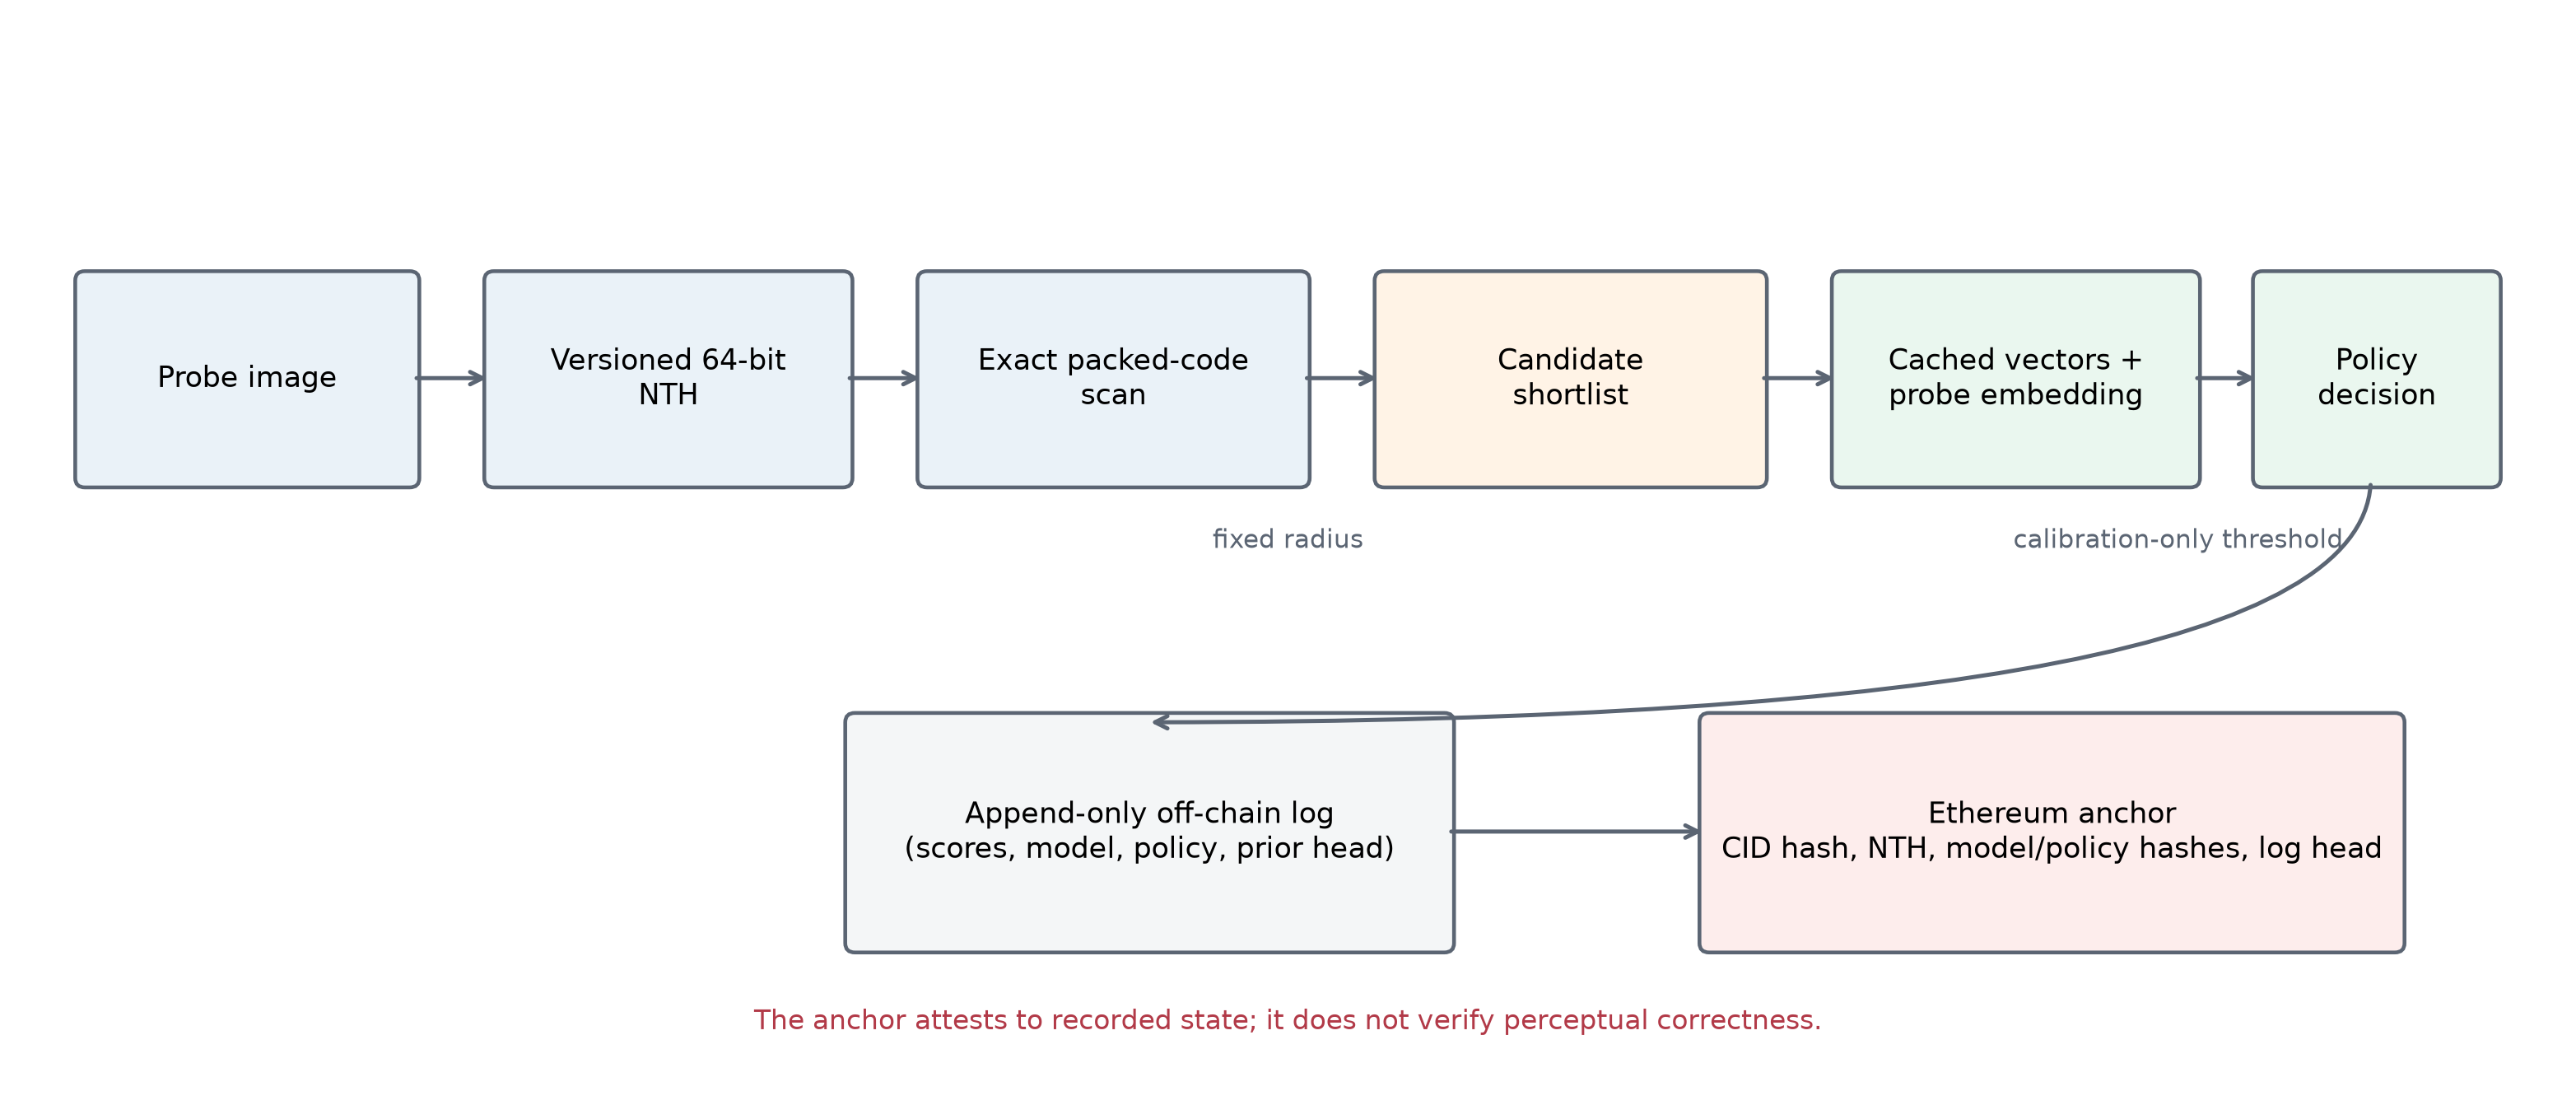
\includegraphics[width=\textwidth]{../figures/revised_system_architecture.png}
\caption{Revised registry architecture. Perceptual computation remains off-chain. The contract attests to versioned recorded state but cannot verify the correctness of a similarity decision.}
\label{fig:architecture}
\end{figure}

The considered adversary may alter an image, submit a prior work, edit unanchored off-chain storage, replay a commitment, or attempt an unauthorised audit-head update. Cryptographic pre-image attacks and consensus-layer failures are outside scope. Anchoring limits undetected post-anchor modification; it cannot prevent pre-anchor omission, a malicious policy, loss of off-chain content, or an incorrect model output.

\subsection{Versioned Neighborhood Totality Hash}

For image $I$, grayscale conversion followed by antialiased Lanczos resizing gives $G\in[0,255]^{8\times8}$. The canonical configuration is named \texttt{nth-v2-exclude-center}. With toroidal indexing, the eight-neighbour sum is
\begin{equation}
  s_{ij}=\sum_{u=-1}^{1}\sum_{v=-1}^{1}G_{(i+u)\bmod8,(j+v)\bmod8}-G_{ij}.
\end{equation}
Let $\bar{s}=64^{-1}\sum_{i,j}s_{ij}$. The bit at $(i,j)$ is $b_{ij}=\mathbb{1}[s_{ij}\geq\bar{s}]$, and row-major packing yields 64 bits. Centre inclusion, reflection, replication, constant padding, global median, adaptive local mean, nearest/bilinear/bicubic interpolation, and $12\times12$/$16\times16$ grids are evaluated separately. The version identifier prevents two implementations from silently producing different commitments.

For an affine photometric transform $G'=aG+b$, $a>0$, the neighbourhood values and their mean transform as $s'_{ij}=as_{ij}+8b$ and $\bar{s}'=a\bar{s}+8b$; therefore the bit comparison is unchanged absent clipping. This does not establish robustness to crop, rotation, nonlinear editing or adversarial perturbation. Those cases are empirical tests.

\subsection{Visual representations and learned controls}

Frozen public weights were used for all six encoder baselines. Output vectors were $\ell_2$ normalised and compared by cosine distance $d_E=1-z_a^\top z_b$. Model selection among frozen encoders used calibration recall at target pair FPR $10^{-3}$, with calibration average precision as a tie-breaker.

The submitted ``NTH-EmbedNet'' name is discontinued because NTH bits were never input to the neural network. The revised control is a MobileNetV3 feature projection: frozen 960-dimensional features pass through a $960\rightarrow512\rightarrow256$ head with batch normalisation, ReLU and unit normalisation. Fixed margins 0.5, 1.0 and 1.5 and an adaptive-margin schedule were screened without test access. Fixed margin 1.5 and the adaptive schedule were each run with seeds 11, 23, 37, 53 and 71. A separate supervised 64-bit hash head uses a pairwise logistic similarity loss, quantisation penalty and balance penalty on frozen MobileNetV3 features. It is a controlled learned-binary baseline, not a reimplementation claim for DSH or HashNet.

\subsection{Calibration and fixed-gate curves}

For negative calibration distances $D^-_{\mathrm{cal}}$ and target $\alpha=10^{-3}$, the threshold is selected automatically as
\begin{equation}
 \tau^*=\max\left\{t:\frac{1}{|D^-_{\mathrm{cal}}|}\sum_{d\in D^-_{\mathrm{cal}}}\mathbb{1}[d\leq t]\leq\alpha\right\}.
\end{equation}
Unique observed values and cumulative tie counts are used; if no observed value satisfies the constraint, the threshold is set immediately below the smallest value. Test labels are not used for threshold or model selection.

At fixed NTH radius $r$, a pair is accepted when
\begin{equation}
  d_H\leq r\quad\land\quad d_E\leq\tau_r.
\end{equation}
For each fixed $r$, the operational curve begins with no accepted pairs and then visits the unique embedding scores of gate-passing pairs in descending order, accepting score ties together. Gate-rejected pairs are excluded from this threshold sequence rather than assigned a recoverable sentinel. The curve therefore terminates after all gate-passing pairs are accepted: its maximum recall is the NTH positive pass rate and its maximum FPR is the NTH negative pass rate. The reported attainable average precision integrates only from zero to this maximum recall. This construction corrects the submitted curve and avoids the artificial terminal $(1,1)$ point added by generic ROC routines.

\subsection{Pair and registry metrics}

Pair FPR is $FP/(FP+TN)$. In a registry with $N$ entries, the more relevant event is that a query accepts at least one wrong entry. We measure this directly for every query rather than infer it from independence:
\begin{equation}
  P_{\mathrm{query,false}}=\frac{1}{Q}\sum_{q=1}^{Q}\mathbb{1}\!\left[\sum_{j\ne y_q}\widehat{y}_{qj}>0\right].
\end{equation}
We also report the mean and 95th-percentile stage-one shortlist, final accepted-candidate count, and true-entry recall.

With cached registry embeddings, per-probe work is
\begin{equation}
 C_{\mathrm{probe}}=C_H(N)+C_E+K_r C_d,
\end{equation}
where $C_H(N)$ is hash lookup, $C_E$ is one probe embedding, $K_r$ is shortlist size, and $C_d$ is one vector distance. NTH reduces comparisons from $N$ to $K_r$ but does not avoid probe inference in this workflow.

\subsection{Data audit and splits}

The authoritative HPC main table contains 91,504 declared pairs from 1,064 seed identities: 29,792 positives and 61,712 negatives. A file-level audit resolved all 1,064 originals and every transformed reference (zero missing originals, transformed references or positive transforms). The smaller local media mirror is therefore not used to define corpus completeness. A deterministic seed-disjoint split (seed 20260830) assigns 745 identities to training, 160 to calibration and 159 to test. Evaluation contains 4,480 calibration positives and 4,452 test positives. Five deterministic within-split negatives are sampled per positive, giving 22,400 and 22,260 negative comparisons respectively. All paths, seed assignments, existence flags and checksums are saved in the full-corpus manifests.

The supplied COCO and Copydays folders are incomplete subsets with renamed files. We evaluate their available images only as seed-source transfer under the same synthetic edit generator: 1,834 COCO-source and 879 Copydays-source positives are usable. This is not the official COCO task \cite{lin2014coco} or Copydays copy-detection protocol \cite{jegou2008copydays}. Separately, the frozen pipeline is evaluated on the official Copydays strong protocol with 157 original references and 229 strong queries. Copydays labels are not used for threshold calibration, and the optional large distractor collections are not included.

\subsection{Implementation and statistical analysis}

The canonical implementation is Python 3.12 with exact local-CPU and HPC locks. Comparative representation experiments used PyTorch 2.13 CPU and torchvision 0.28 on Windows 11 with an Intel Core i7-14700 (28 logical processors); full-corpus verification used PyTorch 2.8.0 and torchvision 0.23.0 on an institutional HPC CPU node. No reported result uses a CUDA timing run. Frozen-model confidence intervals use 2,000 cluster-bootstrap samples at transformed source identity level. Projection and binary-hash variability is reported across five independent seeds. The calibration-selected frozen model and projection replicate are compared on test positives using an exact paired McNemar test.

The 64-bit index is a contiguous packed array using XOR and byte-popcount lookup. Synthetic uniformly random 64-bit codes benchmark exact-scan latency at $10^3$--$10^6$ entries; their shortlist counts are not interpreted as image-data accuracy. Contract gas is measured using Solidity 0.8.24 with optimiser (200 runs) on a deterministic PyEVM local chain.

\color{black}
\section{Results}
% REVIEWERS: all quantitative and robustness requests
\color{revisionred}

\subsection{Hash baselines and ablations}

Table~\ref{tab:hashes} applies the same calibration rule to each 64-bit hash on the complete main corpus. NTH-default did not outperform pHash or dHash in held-out recall. Adaptive thresholding improved NTH recall from 0.6548 to 0.6833, but pHash remained higher at 0.7224. A $16\times16$ NTH grid reached 0.6799 recall with test FPR 0.000674. Zero padding was the weakest boundary rule (recall 0.4573, FPR 0.00315). Bilinear and bicubic interpolation exceeded the target on test, whereas the antialiased Lanczos default remained closer to it.

\begin{table}[ht]
\centering
\caption{Held-out hash performance after calibration to pair FPR $\leq10^{-3}$.}
\label{tab:hashes}
\begin{tabular}{lrrr}
\toprule
Method & Radius & Recall & Test FPR\\
\midrule
aHash & 6 & 0.6512 & 0.000494\\
dHash & 14 & 0.7053 & 0.000404\\
pHash & 16 & 0.7224 & 0.000404\\
wHash-Haar & 7 & 0.6417 & 0.000539\\
NTH-default & 4 & 0.6548 & 0.000764\\
NTH-adaptive & 9 & 0.6833 & 0.000898\\
NTH-$12\times12$ & 13 & 0.6831 & 0.001213\\
NTH-$16\times16$ & 27 & 0.6799 & 0.000674\\
\bottomrule
\end{tabular}
\end{table}

Full-registry curves (Fig.~\ref{fig:hashtradeoff}) likewise show no uniformly dominant compact hash. At approximately 0.90 true-candidate recall, NTH used radius 15 and averaged 69.8 candidates, while aHash used radius 18 and averaged 51.8. NTH was more selective than dHash and pHash at this target but not more selective than aHash or wHash. The revised conclusion is therefore that NTH is one versioned gate with measurable behaviour, not a generally superior perceptual hash.

\begin{figure}[ht]
\centering
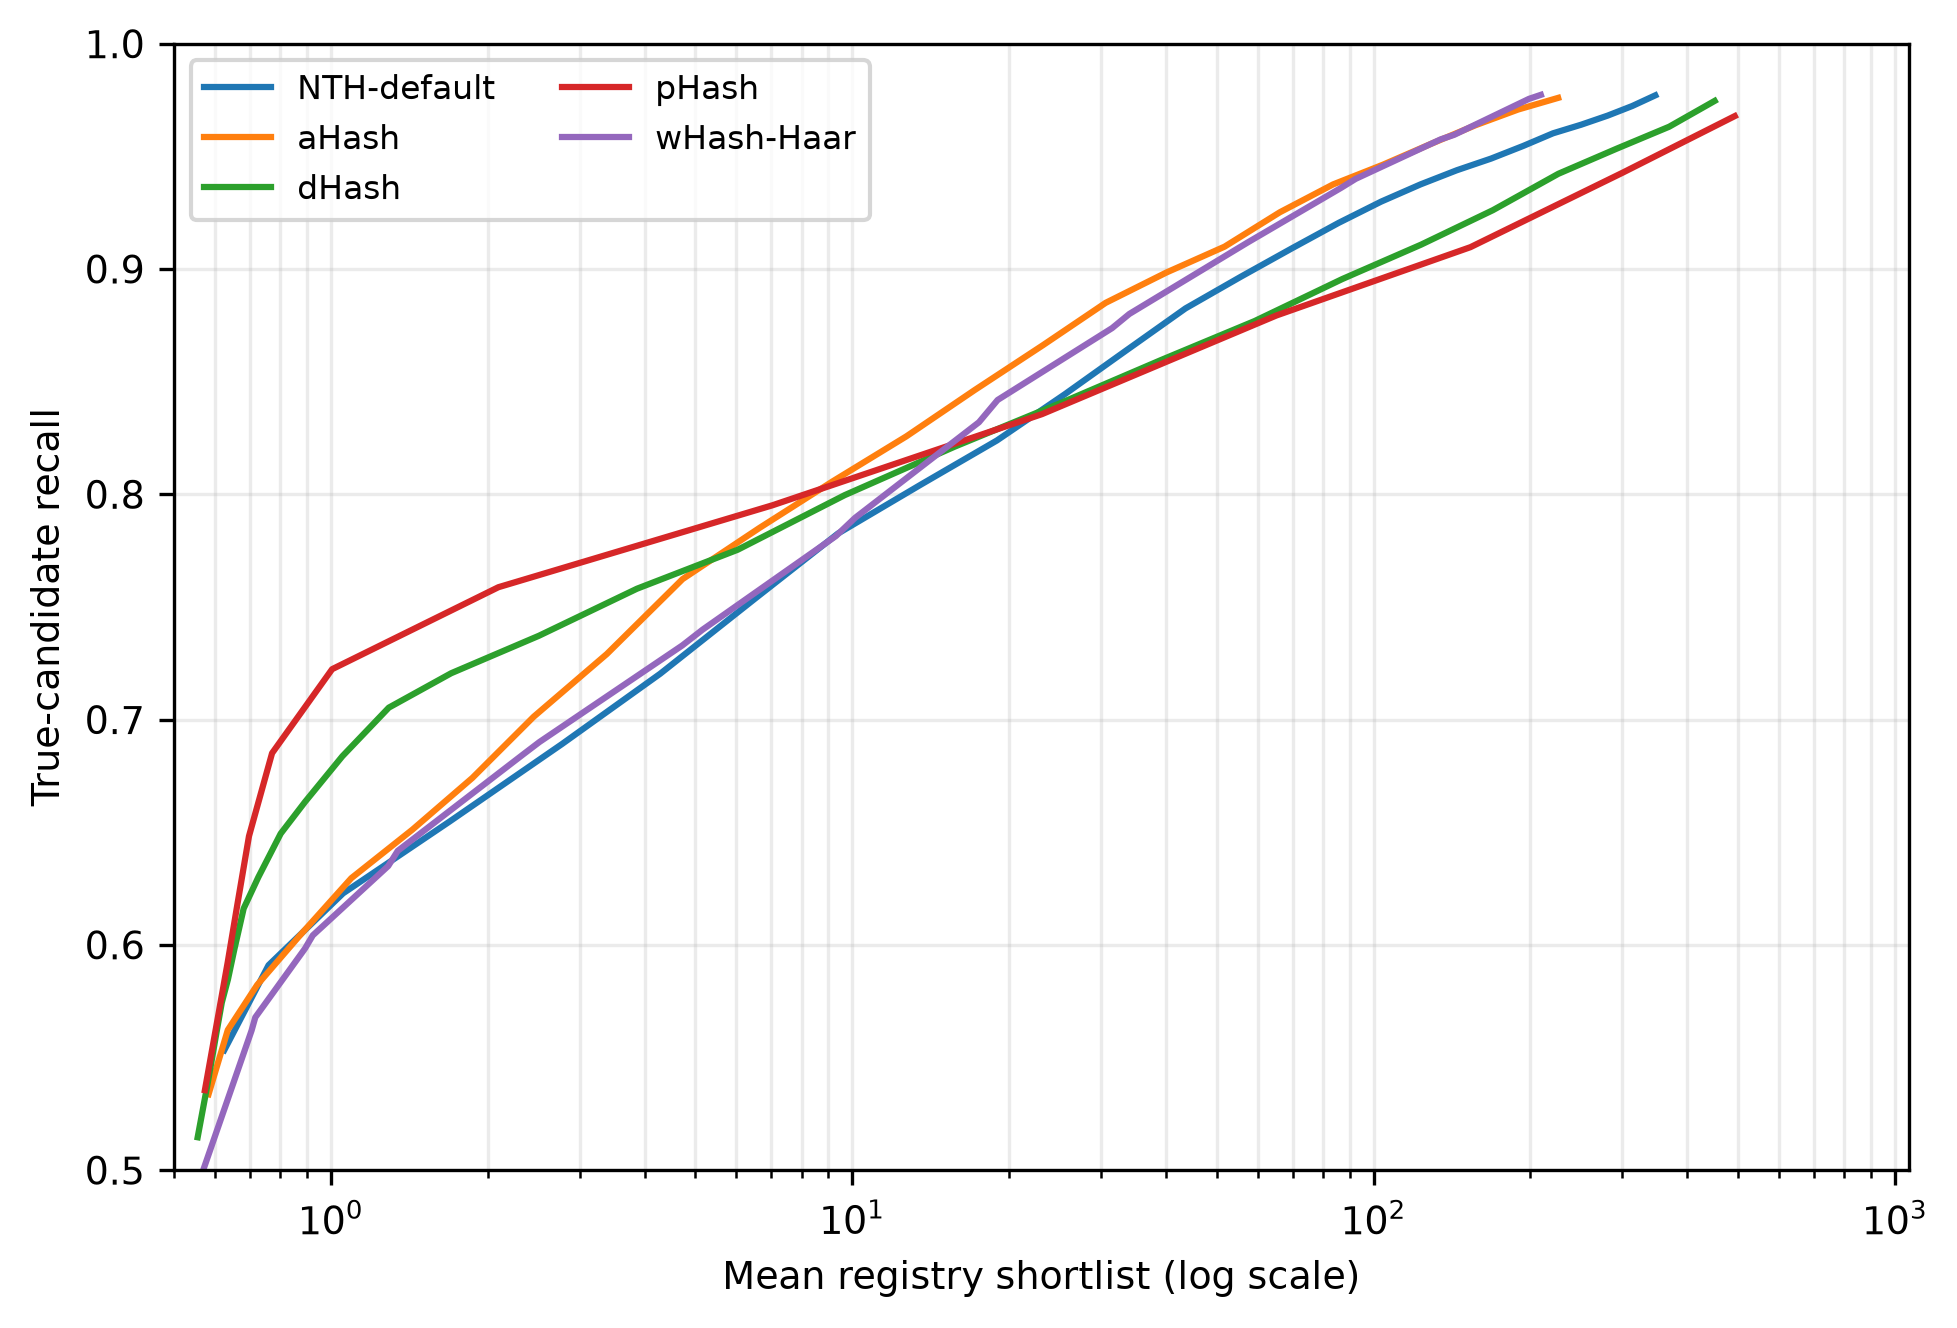
\includegraphics[width=0.72\textwidth]{../figures/hash_registry_tradeoff.png}
\caption{True-candidate recall versus mean shortlist for the five 64-bit methods on the 1,064-entry registry.}
\label{fig:hashtradeoff}
\end{figure}

\subsection{Modern encoders and learned controls}

The six-encoder comparison on the deterministic local mirror selected ShuffleNet V2 from calibration performance and gave held-out recall 0.9681 (cluster-bootstrap 95\% CI 0.9561--0.9791) with FPR 0.000074. EfficientNet-B0 was close at recall 0.9637. DINOv2 and CLIP were strong by AUC/AP but less sensitive at this extreme low-FPR operating point (Table~\ref{tab:deep}). We then reran the selected ShuffleNet model on every resolved main-corpus image at the HPC: recall was 0.9681 (95\% CI 0.9589--0.9762), FPR 0.000359 and AP 0.99898. This complete-corpus result is used for the subsequent two-stage analysis and shows that the selected model's recall is stable to restoration of the local mirror's absent files.

\begin{table}[ht]
\centering
\caption{Frozen encoder results under the common calibration/test protocol. The first row is the complete private main corpus; the six-model selection comparison below it used the deterministic local mirror.}
\label{tab:deep}
\begin{tabular}{lrrrr}
\toprule
Encoder & Test recall & 95\% CI & Test FPR & AP\\
\midrule
\multicolumn{5}{l}{\emph{Complete private main-corpus verification}}\\
ShuffleNet V2 1.0x & 0.9681 & [0.9589, 0.9762] & 0.000359 & 0.99898\\
\addlinespace
\multicolumn{5}{l}{\emph{Six-encoder comparison on deterministic local mirror}}\\
ShuffleNet V2 1.0x & 0.9681 & [0.9561, 0.9791] & 0.000074 & 0.99897\\
EfficientNet-B0 & 0.9637 & [0.9505, 0.9760] & 0.000148 & 0.99917\\
ResNet-50 & 0.9355 & [0.9159, 0.9539] & 0.000742 & 0.99846\\
MobileNetV3-Large & 0.9295 & [0.9102, 0.9500] & 0.000742 & 0.99856\\
DINOv2 ViT-S/14 & 0.8609 & [0.8342, 0.8855] & 0.000074 & 0.99817\\
CLIP ViT-B/32 & 0.8550 & [0.8227, 0.8854] & 0.000371 & 0.99453\\
\bottomrule
\end{tabular}
\end{table}

Five fixed-margin projection runs obtained mean recall $0.9130\pm0.0142$ and mean FPR $0.000445\pm0.000074$. Adaptive margins reduced mean recall to $0.8923\pm0.0203$. The frozen MobileNetV3 features themselves reached 0.9295 recall. The calibration-selected fixed-margin replicate was also inferior to ShuffleNet V2 on paired test positives (173 pairs correct only for ShuffleNet versus 51 only for the projection; exact two-sided $p=1.02\times10^{-16}$). Thus, the projection training did not establish a contribution. The supervised 64-bit learned hash was unstable across five seeds (recall $0.5574\pm0.1022$) and is retained as a negative control.

\subsection{Fixed-gate registry trade-off}

Figure~\ref{fig:performance} and Table~\ref{tab:twostage} report the complete-corpus NTH--ShuffleNet system. At $r=16$, the gate reduced mean embedding comparisons from 1,064 to 85.7 (91.9\%) but capped test recall at 0.9205 before embedding confirmation and produced 0.9030 end-to-end recall. The full-registry probability of any false accepted entry was 0.1929, with pair FPR 0.000135. At $r=12$, mean comparisons fell to 33.7 and the false-query probability was 0.2102, but recall was 0.8565. There is no single universally optimal radius; it is a deployment policy determined by the cost of missed registrations and comparisons.

\begin{table}[ht]
\centering
\caption{Held-out two-stage results with fixed NTH radius and a calibration-only ShuffleNet threshold.}
\label{tab:twostage}
\begin{tabular}{rrrrrr}
\toprule
$r$ & Pair recall & Pair FPR & Any false/query & Mean shortlist & Final accepted\\
\midrule
2  & 0.5910 & 0.000000 & 0.0840 & 0.76 & 0.70\\
4  & 0.6548 & 0.000764 & 0.3203 & 1.69 & 1.65\\
8  & 0.7814 & 0.000809 & 0.2850 & 9.39 & 2.04\\
12 & 0.8565 & 0.000404 & 0.2102 & 33.67 & 1.54\\
16 & 0.9030 & 0.000135 & 0.1929 & 85.73 & 1.45\\
\bottomrule
\end{tabular}
\end{table}

Deep-only ShuffleNet compared all 1,064 vectors, reached recall 0.9681 and had directly measured any-false/query probability 0.2758. The $r=16$ two-stage configuration reduced mean comparisons to 85.7 and any-false/query probability to 0.1929, but lost 6.5 percentage points of recall. This is the central operational trade-off, replacing the submitted claim that the first stage simply avoids most embedding inference.

\begin{figure}[ht]
\centering
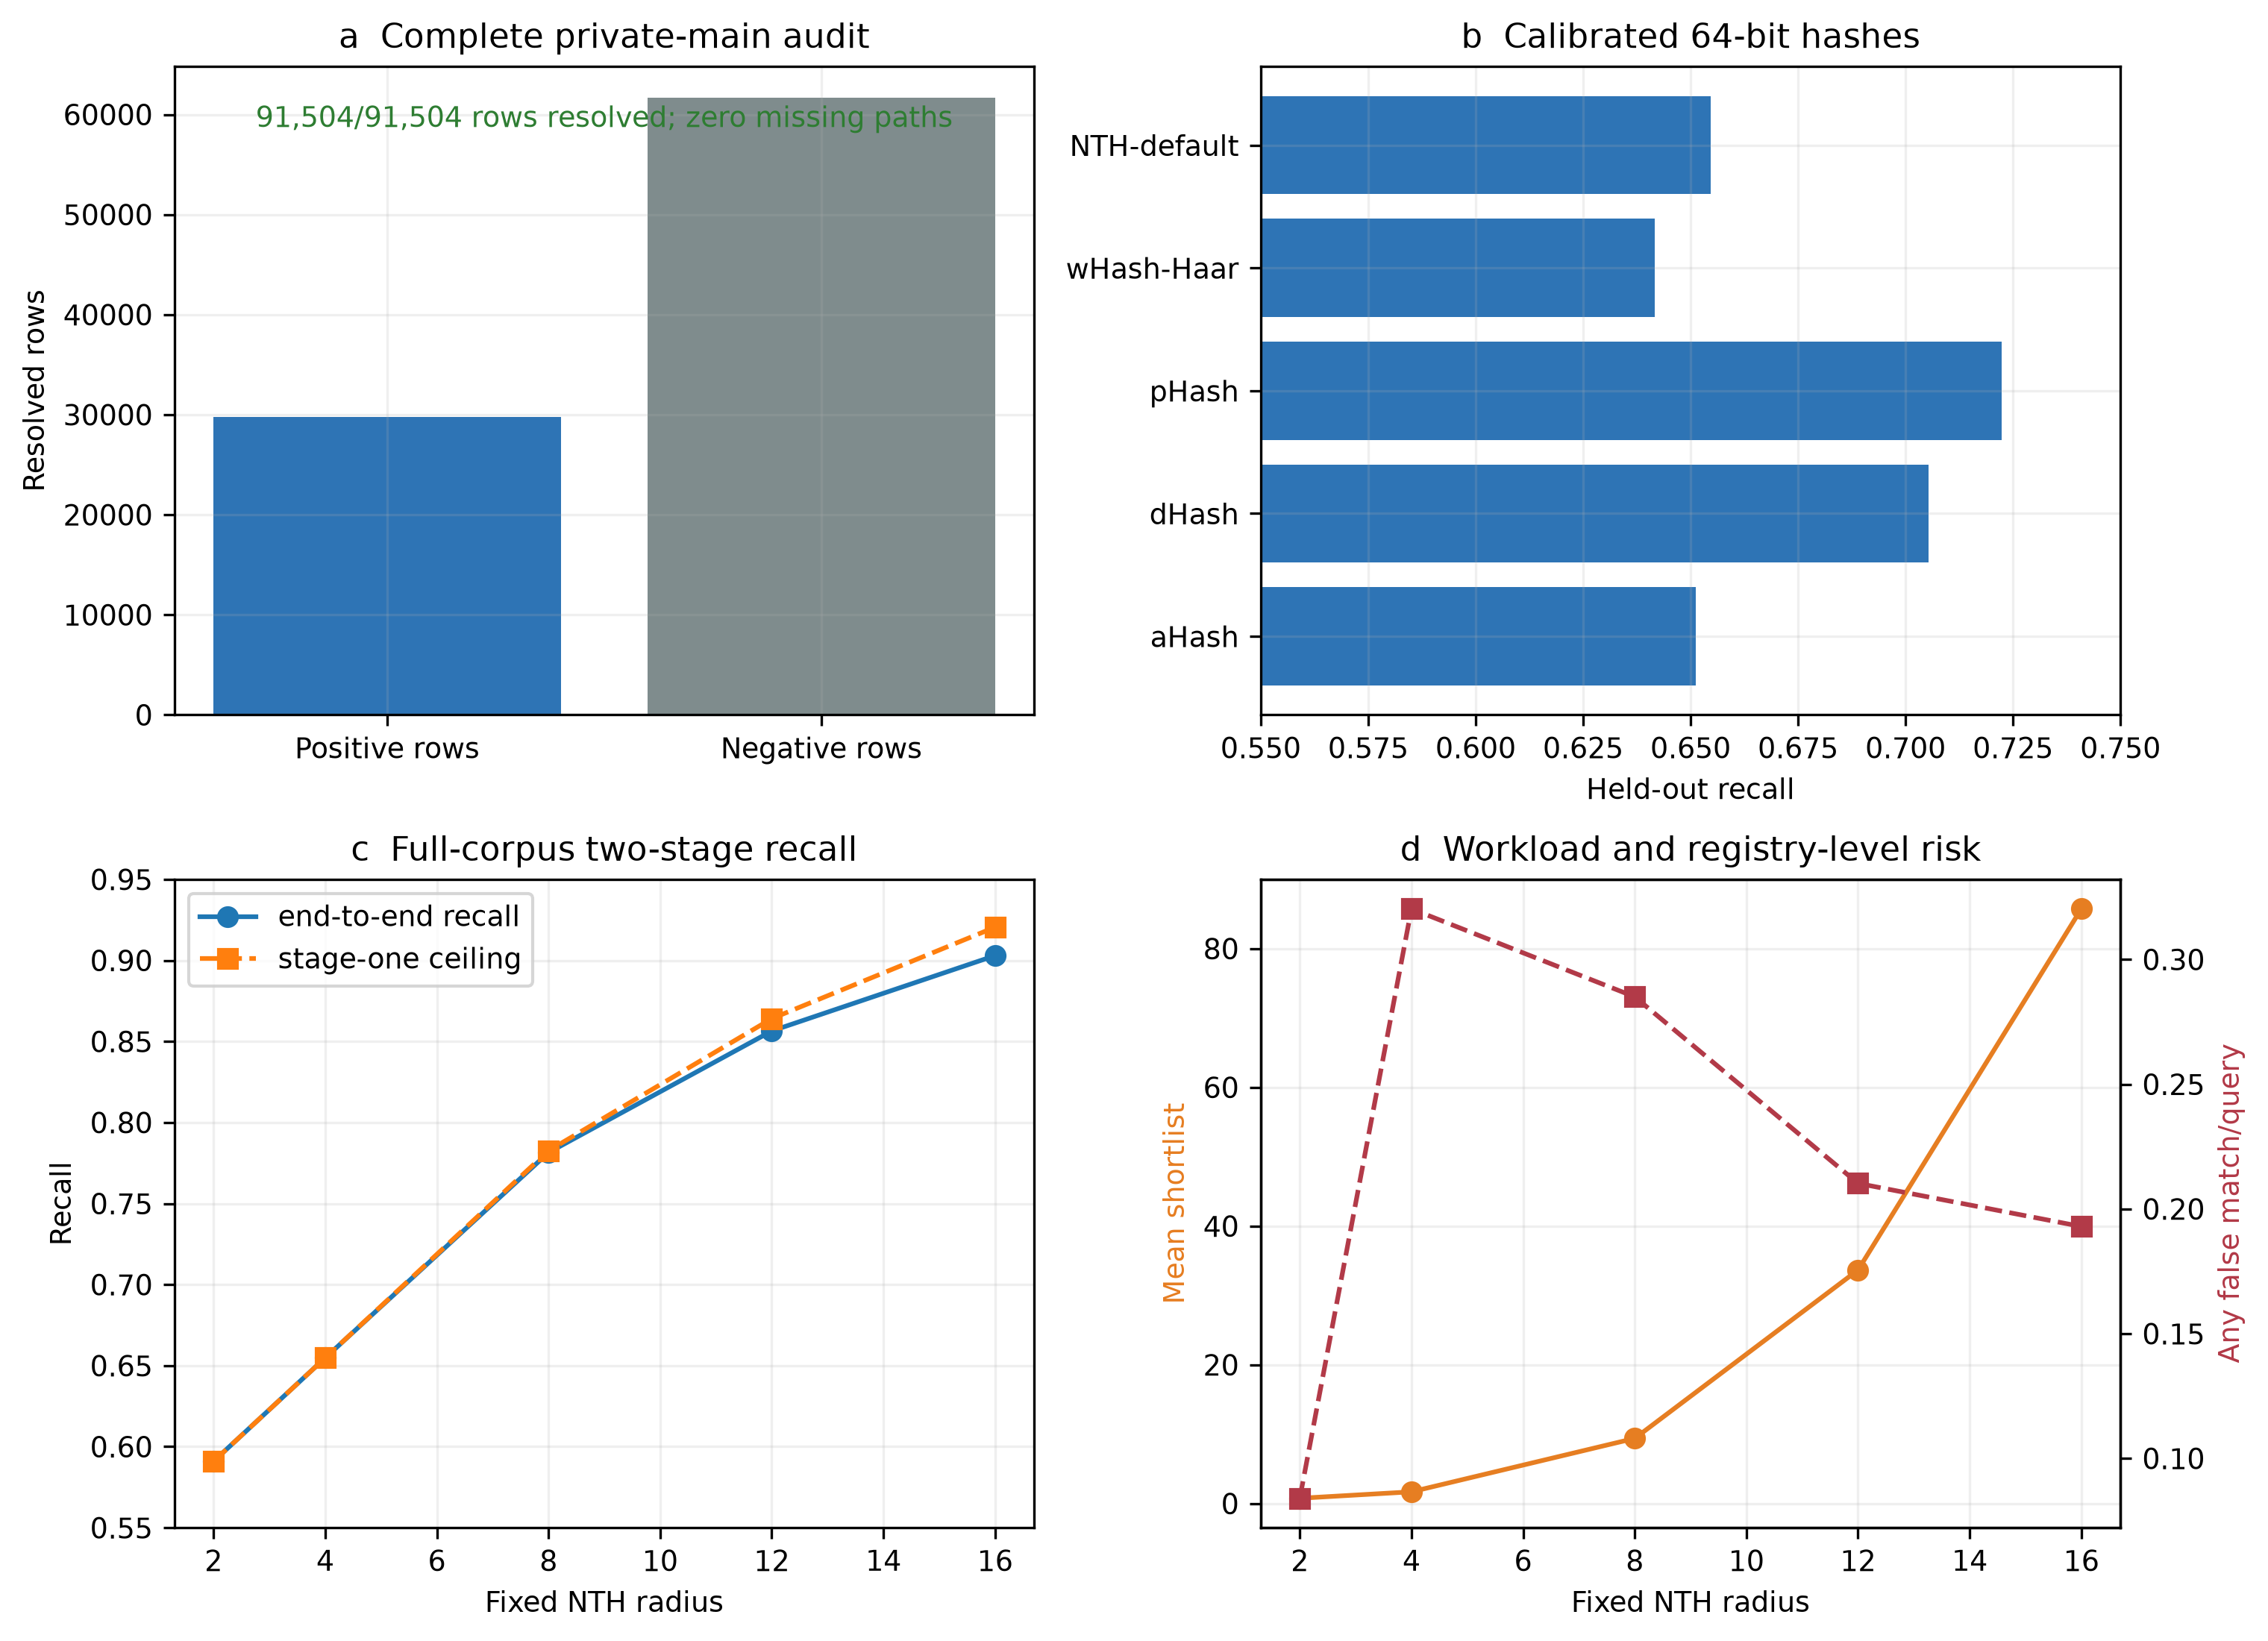
\includegraphics[width=\textwidth]{../figures/full_main_verification_summary.png}
\caption{Complete private-main-corpus audit, classical-hash comparison and fixed-gate registry trade-offs. The selected-model confidence interval is clustered by transformed source identity.}
\label{fig:performance}
\end{figure}

Fixed-gate ROC curves were generated separately for each radius on a logarithmic FPR axis. Their maximum recall equals the corresponding NTH pass rate, as required by the decision rule; none is allowed to recover rejected positives by changing $r$ during a sweep.

\subsection{Transfer, crop and bounded perturbations}

Using thresholds selected only on the main calibration split, ShuffleNet-only recall was 0.9618 on 1,834 available COCO-source positives and 0.9693 on 879 Copydays-source positives. NTH $r=16$ plus ShuffleNet reached 0.8860 and 0.9238 respectively. Because the same synthetic edit generator was used and the supplied benchmark folders are incomplete, these numbers demonstrate only source-image transfer.

The official Copydays evaluation produced materially lower transfer performance (Table~\ref{tab:copydays}). ShuffleNet ranked the correct original first for 0.7031 of strong queries and within the first five for 0.8690; mean reciprocal rank and mean average precision were both 0.7770 because each query has one relevant original. At the embedding threshold frozen on the private main calibration split, however, only 0.2402 of true matches were accepted. The NTH $r=16$ gate admitted the true identity for 0.4454 of queries and the complete two-stage policy accepted 0.1921. These negative results demonstrate domain shift and prevent a claim of benchmark-level generality.

\begin{table}[ht]
\centering
\caption{Official Copydays strong-query evaluation. Thresholds were frozen on the private main calibration split; 157 original references and 229 strong queries were used without optional distractors.}
\label{tab:copydays}
\begin{tabular}{lrrrr}
\toprule
Policy & Top-1 retrieval & Recall@5 & True acceptance & Any false/query\\
\midrule
ShuffleNet only & 0.7031 & 0.8690 & 0.2402 & 0.00437\\
NTH $r=16$ + ShuffleNet & 0.1921 & -- & 0.1921 & 0.00437\\
\bottomrule
\end{tabular}
\end{table}

At the calibrated NTH-only radius 4, central crop followed by resize reduced recall from 1.0 with no crop to 0.679, 0.233, 0.107, 0.031 and 0.006 when 10, 20, 30, 40 and 50\% were removed from both width and height. We therefore implemented an off-chain multiview reference bank containing the full image plus fixed central crops at 10, 20, 30, 40 and 50\%. Queries used held-out crop ratios of 15, 25, 35 and 45\%, so no query view was copied into the bank. For NTH $r=16$ plus ShuffleNet, true acceptance improved from 0.9748, 0.8176, 0.6101 and 0.3019 with one reference view to 1.0 at all four ratios with six views. The directly measured any-false/query probability also changed from 0.0440, 0.0377, 0.0314 and 0.0063 to 0.0881, 0.0818, 0.0566 and 0.0503. Thus multiview storage is a concrete off-chain mitigation, not a free robustness gain. On-chain storage remains unchanged because the registry anchors the model/policy identifiers and audit head rather than every reference embedding.

For each of 159 test originals and perturbation budget $\epsilon\in\{1,2,4,8,16\}$, 32 black-box trials maximised NTH distance. Independent pixelwise Rademacher noise caused no evasion at radius 4, but coherent $8\times8$ masks caused evasion rates 0.006, 0.031, 0.182, 0.484 and 0.843. This experiment is not a complete adversarial evaluation; it is evidence that low-frequency structured perturbations are a practical weakness.

An additional adaptive score-query coordinate search targeted the canonical $8\times8$ luminance grid consumed by NTH. Across all 159 test identities and 256 NTH queries per image/budget, the radius-4 evasion rate was 0, 0.0063, 0.0314 and 0.1069 at grid-domain $L_\infty$ budgets 1, 2, 4 and 8, respectively. This attack adapts to the actual NTH score but acts after Lanczos preprocessing; it is neither a source-pixel guarantee nor a certified adversarial bound.

\subsection{Index, inference and contract measurements}

Figure~\ref{fig:stress} summarises failure and scale tests. Vectorised exact scan averaged 0.042, 0.272, 3.58 and 38.46 ms for $10^3$, $10^4$, $10^5$ and $10^6$ random codes, with 8 MB of code storage at $10^6$. These CPU results should not be extrapolated to distributed or approximate indexes without measurement.

The selected ShuffleNet V2 encoder was re-benchmarked on two additional hardware platforms for batch sizes 1, 8, 32 and 64 with ten timed repetitions after three warm-up batches. On an Intel Core i7-14700 workstation CPU, median latency was 13.00, 2.89, 2.62 and 2.78 ms/image, and throughput peaked at 382.2 images/s for batch 32. On a 16-core allocation of an Intel Xeon Gold 5320 HPC node, median latency was 9.78, 1.98, 1.24 and 1.25 ms/image, and throughput peaked at 805.6 images/s for batch 32. MobileNetV3 and EfficientNet-B0 were also measured on the local CPU by the same script. Thirteen canonical unit tests were verified locally and on the versioned HPC working copy, and the complete main-corpus audit and selected-model verification ran on an HPC CPU node. An A100 timing run was deliberately not reported because the shared device was at 100\% utilisation (73.7/81.9 GB occupied by unrelated multi-user processes), which would invalidate a clean benchmark. The workstation is a CPU proxy rather than a dedicated embedded edge device, so no mobile-edge latency claim is made.

The revised Solidity contract used 183,064--183,076 gas for registration at registry sizes 0, 1, 10, 100 and 1,000, consistent with constant-size mapping insertion. Updating the audit head used 31,905 gas; deployment used 360,358 gas. Duplicate commitments, zero CID hashes and unauthorised head updates reverted. These are local-EVM gas units, not mainnet prices.

\begin{figure}[ht]
\centering
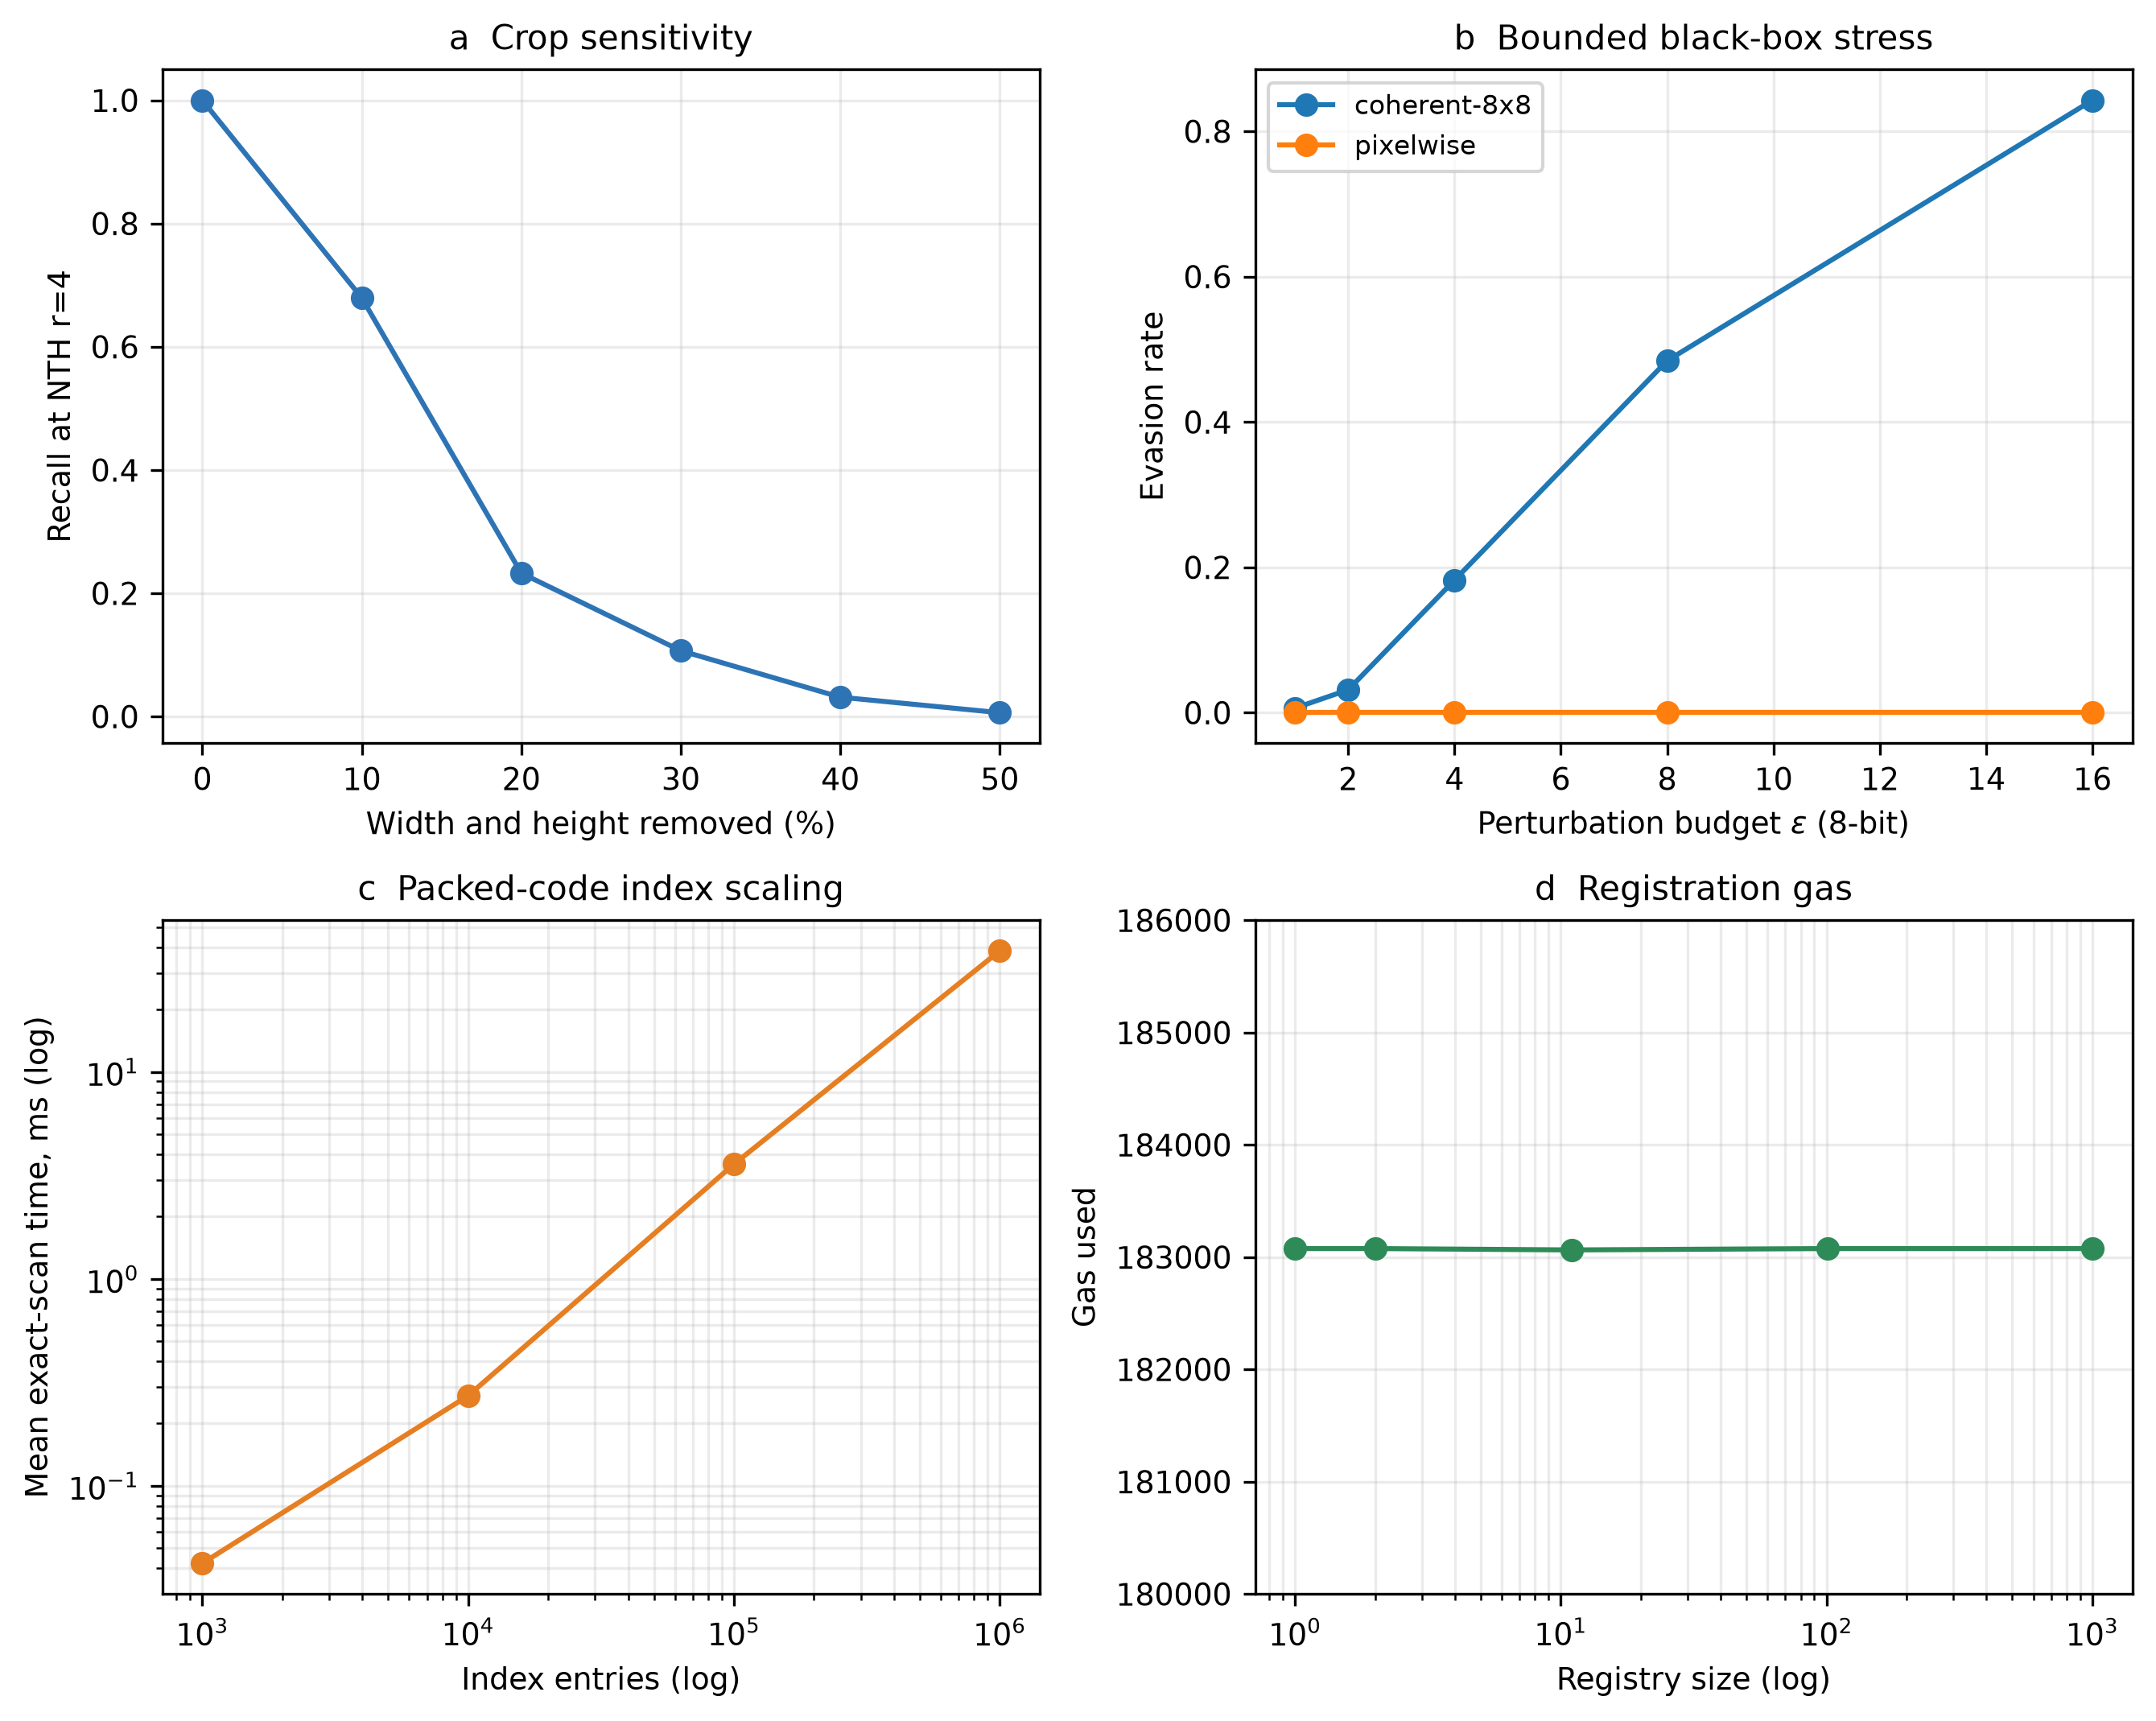
\includegraphics[width=0.9\textwidth]{../figures/stress_and_scaling.png}
\caption{Crop sensitivity, bounded black-box evasion, exact packed-code scan latency and local-EVM registration gas.}
\label{fig:stress}
\end{figure}

\color{black}
\section{Discussion}
% REVIEWERS: R2.1; R2.4; R3.3; R4.4; R5.4; R6.5; R7.5
\color{revisionred}

The revised evidence supports a narrower claim than the submitted manuscript. A compact gate can reduce the number of embedding comparisons, but the best tested frozen encoder already performs strongly, and the gate creates a hard recall ceiling. Furthermore, pair FPR below $10^{-3}$ can coexist with a query-level false-match probability above 0.2 in a 1,064-entry registry because each query creates many opportunities for an incorrect acceptance. Registry policies should therefore be calibrated and reported at the intended index scale.

NTH should be viewed as an engineering construction in the block/local-statistics family. Its wrap-around, threshold and resolution choices are now measurable and versioned, but the experiments do not establish a new hashing paradigm or general superiority. At high target recall, aHash and wHash produced smaller shortlists; at a strict pair operating point, pHash and dHash obtained higher recall. The retained value of NTH is a simple reproducible gate whose behaviour can be audited, not an accuracy claim.

Likewise, the neural results argue against naming a standard projection as a novel network. Frozen ShuffleNet and EfficientNet were strongest, while task-specific projection reduced recall and adaptive margins did not help. This negative result is scientifically useful because it shows that near-perfect AUC on constructed pairs can obscure model-ranking differences in the low-FPR region.

The contract improves tamper evidence by anchoring model, policy and log-head hashes, but it does not make an off-chain decision trustless. A complete dispute process needs public artefacts, deterministic recomputation, retained off-chain objects, defined contract governance and rules for upgrades. Before anchoring, an operator can omit events or select a misleading policy. After anchoring, the chain reveals alteration but cannot recover lost logs or decide which perceptual model is legitimate.

\color{black}
\section{Limitations}
% REVIEWERS: limitations requested across R1-R7
\color{revisionred}

The largest limitation is public data provenance. Although the private HPC corpus resolves all 91,504 pair-table references and all 1,064 pre-rename filenames were recovered from notebook output, the constructed images still lack author-confirmed source URLs, owners and licences. They cannot responsibly be redistributed until those records are resolved, so an independent reader cannot yet reconstruct the exact private-media experiment from the proposed public package. The renamed local COCO/Copydays subsets remain only source-transfer checks. The separate official Copydays strong evaluation omits optional large distractor sets and exposed substantial domain shift.

Timing is now measured on workstation and server CPUs, but not on a dedicated embedded edge accelerator. The bounded-noise and adaptive score-query studies are finite diagnostics, not certified robustness, and the adaptive attack is defined on the post-resampling NTH grid rather than source pixels. The multiview crop fallback uses six off-chain references per identity and increases false-match exposure; broader geometric alignment remains untested. The exact index benchmark uses random codes and does not model network, persistence or multi-user concurrency. At million-scale, approximate or multi-index methods may be preferable. No user study or operational dispute evaluation was performed. Finally, local EVM gas is reproducible but does not capture mainnet fees, congestion, rollups or governance.

\color{black}
\section{Conclusion}
% REVIEWERS: editor; R2.1-R2.2; R7.1
\color{revisionred}

This revision replaces overstated performance and audit claims with a reproducible systems analysis. The strongest tested frozen encoder outperformed the learned projection. NTH reduced vector comparisons but imposed a substantial recall ceiling and was not uniformly better than classical hashes. Query-level evaluation showed why pair FPR cannot be interpreted as registry risk, while crop and structured-noise tests exposed practical weaknesses. The revised contract provides versioned tamper evidence, not on-chain perceptual verification. A deployer may still choose a compact gate when comparison cost is critical, but that choice must be made from fixed-radius recall, shortlist and registry false-match measurements rather than global AUC alone.

\color{black}
\section*{Data availability}
% REVIEWERS: R4.5; R5.1; R7.2
\color{revisionred}

Pair manifests, deterministic split lists, file-level audit tables, result tables, the recovered 1,064-file rename register and source-code checksums are included in the versioned reproducibility package. The complete private HPC corpus was used for the main file audit and full-corpus verification, but author-confirmed source provenance and licences remain incomplete; therefore the private media are not redistributed. Official Copydays original/strong images were used locally under the benchmark's INRIA copyright notice and are also not redistributed; archive checksums and aggregate/query results are supplied. The versioned reproducibility package is available at DOI: \texttt{\RepositoryDOI}.

\section*{Code availability}

The canonical NTH implementation, evaluation scripts, tests, contract, environment files and result-generation commands are available in the versioned reproducibility package at DOI: \texttt{\RepositoryDOI}. Historical scripts containing credentials and media without verified redistribution rights are excluded from the release.

\color{black}
\section*{Author contributions}

Conceptualization, methodology, model development, dataset preparation, and writing--original draft: Stuti Pandey. Investigation, validation, blockchain integration, and writing--review and editing: Akhilendra Pratap Singh. Supervision, validation, and technical guidance: Dharmender Singh Kushwaha. Conceptualization, supervision, and system integration: Ashish Pandey. All authors reviewed and approved the final manuscript.

\section*{Funding}

The authors declare that no funds, grants, or other support were received.

\section*{Ethics approval and consent to participate}

Not applicable. The study evaluates image-processing software and does not report research involving human participants or identifiable personal data.

\section*{Consent for publication}

Not applicable.

\section*{Competing interests}

The authors declare no competing interests.

\bibliographystyle{unsrt}
\bibliography{ref_revised}

\end{document}
